\documentclass[twoside]{book}

% Packages required by doxygen
\usepackage{calc}
\usepackage{doxygen}
\usepackage{graphicx}
\usepackage[utf8]{inputenc}
\usepackage{makeidx}
\usepackage{multicol}
\usepackage{multirow}
\usepackage{textcomp}
\usepackage[table]{xcolor}

% Font selection
\usepackage[T1]{fontenc}
\usepackage{mathptmx}
\usepackage[scaled=.90]{helvet}
\usepackage{courier}
\usepackage{amssymb}
\usepackage{sectsty}
\renewcommand{\familydefault}{\sfdefault}
\allsectionsfont{%
  \fontseries{bc}\selectfont%
  \color{darkgray}%
}
\renewcommand{\DoxyLabelFont}{%
  \fontseries{bc}\selectfont%
  \color{darkgray}%
}

% Page & text layout
\usepackage{geometry}
\geometry{%
  a4paper,%
  top=2.5cm,%
  bottom=2.5cm,%
  left=2.5cm,%
  right=2.5cm%
}
\tolerance=750
\hfuzz=15pt
\hbadness=750
\setlength{\emergencystretch}{15pt}
\setlength{\parindent}{0cm}
\setlength{\parskip}{0.2cm}
\makeatletter
\renewcommand{\paragraph}{%
  \@startsection{paragraph}{4}{0ex}{-1.0ex}{1.0ex}{%
    \normalfont\normalsize\bfseries\SS@parafont%
  }%
}
\renewcommand{\subparagraph}{%
  \@startsection{subparagraph}{5}{0ex}{-1.0ex}{1.0ex}{%
    \normalfont\normalsize\bfseries\SS@subparafont%
  }%
}
\makeatother

% Headers & footers
\usepackage{fancyhdr}
\pagestyle{fancyplain}
\fancyhead[LE]{\fancyplain{}{\bfseries\thepage}}
\fancyhead[CE]{\fancyplain{}{}}
\fancyhead[RE]{\fancyplain{}{\bfseries\leftmark}}
\fancyhead[LO]{\fancyplain{}{\bfseries\rightmark}}
\fancyhead[CO]{\fancyplain{}{}}
\fancyhead[RO]{\fancyplain{}{\bfseries\thepage}}
\fancyfoot[LE]{\fancyplain{}{}}
\fancyfoot[CE]{\fancyplain{}{}}
\fancyfoot[RE]{\fancyplain{}{\bfseries\scriptsize Generated on Thu May 29 2014 18\-:45\-:05 for Swift by Doxygen }}
\fancyfoot[LO]{\fancyplain{}{\bfseries\scriptsize Generated on Thu May 29 2014 18\-:45\-:05 for Swift by Doxygen }}
\fancyfoot[CO]{\fancyplain{}{}}
\fancyfoot[RO]{\fancyplain{}{}}
\renewcommand{\footrulewidth}{0.4pt}
\renewcommand{\chaptermark}[1]{%
  \markboth{#1}{}%
}
\renewcommand{\sectionmark}[1]{%
  \markright{\thesection\ #1}%
}

% Indices & bibliography
\usepackage{natbib}
\usepackage[titles]{tocloft}
\setcounter{tocdepth}{3}
\setcounter{secnumdepth}{5}
\makeindex

% Hyperlinks (required, but should be loaded last)
\usepackage{ifpdf}
\ifpdf
  \usepackage[pdftex,pagebackref=true]{hyperref}
\else
  \usepackage[ps2pdf,pagebackref=true]{hyperref}
\fi
\hypersetup{%
  colorlinks=true,%
  linkcolor=blue,%
  citecolor=blue,%
  unicode%
}

% Custom commands
\newcommand{\clearemptydoublepage}{%
  \newpage{\pagestyle{empty}\cleardoublepage}%
}


%===== C O N T E N T S =====

\begin{document}

% Titlepage & ToC
\hypersetup{pageanchor=false}
\pagenumbering{roman}
\begin{titlepage}
\vspace*{7cm}
\begin{center}%
{\Large Swift \\[1ex]\large 0.\-1 }\\
\vspace*{1cm}
{\large Generated by Doxygen 1.8.6}\\
\vspace*{0.5cm}
{\small Thu May 29 2014 18:45:05}\\
\end{center}
\end{titlepage}
\clearemptydoublepage
\tableofcontents
\clearemptydoublepage
\pagenumbering{arabic}
\hypersetup{pageanchor=true}

%--- Begin generated contents ---
\chapter{R\-E\-A\-D\-M\-E}
\label{md__r_e_a_d_m_e}
\hypertarget{md__r_e_a_d_m_e}{}
S\-W\-I\-F\-T Copyright (c) 2014 Thomas Lextrait \href{mailto:thomas.lextrait@gmail.com}{\tt thomas.\-lextrait@gmail.\-com} All rights reserved

Swift is a simple framework that allows you to design a R\-E\-S\-Tful A\-P\-I in C++. 
\chapter{Namespace Index}
\section{Namespace List}
Here is a list of all documented namespaces with brief descriptions\-:\begin{DoxyCompactList}
\item\contentsline{section}{\hyperlink{namespaceswift}{swift} }{\pageref{namespaceswift}}{}
\end{DoxyCompactList}

\chapter{Hierarchical Index}
\section{Class Hierarchy}
This inheritance list is sorted roughly, but not completely, alphabetically\-:\begin{DoxyCompactList}
\item \contentsline{section}{cgi\-\_\-env\-\_\-block}{\pageref{structcgi__env__block}}{}
\item \contentsline{section}{char64long16}{\pageref{unionchar64long16}}{}
\item \contentsline{section}{connection}{\pageref{structconnection}}{}
\item \contentsline{section}{ctl\-\_\-msg}{\pageref{structctl__msg}}{}
\item \contentsline{section}{dir\-\_\-entry}{\pageref{structdir__entry}}{}
\item \contentsline{section}{endpoint}{\pageref{unionendpoint}}{}
\item exception\begin{DoxyCompactList}
\item \contentsline{section}{swift\-:\-:invalid\-\_\-method\-\_\-exception}{\pageref{classswift_1_1invalid__method__exception}}{}
\item \contentsline{section}{swift\-:\-:null\-\_\-http\-\_\-version}{\pageref{classswift_1_1null__http__version}}{}
\item \contentsline{section}{swift\-:\-:null\-\_\-request\-\_\-exception}{\pageref{classswift_1_1null__request__exception}}{}
\item \contentsline{section}{swift\-:\-:null\-\_\-uri}{\pageref{classswift_1_1null__uri}}{}
\end{DoxyCompactList}
\item \contentsline{section}{swift\-:\-:Header}{\pageref{classswift_1_1_header}}{}
\item \contentsline{section}{swift\-:\-:Hook}{\pageref{classswift_1_1_hook}}{}
\item \contentsline{section}{iobuf}{\pageref{structiobuf}}{}
\item \contentsline{section}{M\-D5\-Context}{\pageref{struct_m_d5_context}}{}
\item \contentsline{section}{mg\-\_\-connection}{\pageref{structmg__connection}}{}
\item \contentsline{section}{mg\-\_\-expansion}{\pageref{structmg__expansion}}{}
\item \contentsline{section}{mg\-\_\-connection\-:\-:mg\-\_\-header}{\pageref{structmg__connection_1_1mg__header}}{}
\item \contentsline{section}{mg\-\_\-iterator}{\pageref{structmg__iterator}}{}
\item \contentsline{section}{mg\-\_\-server}{\pageref{structmg__server}}{}
\item \contentsline{section}{ns\-\_\-connection}{\pageref{structns__connection}}{}
\item \contentsline{section}{ns\-\_\-server}{\pageref{structns__server}}{}
\item \contentsline{section}{swift\-:\-:Request}{\pageref{classswift_1_1_request}}{}
\item \contentsline{section}{swift\-:\-:Response}{\pageref{classswift_1_1_response}}{}
\item \contentsline{section}{swift\-:\-:Server}{\pageref{classswift_1_1_server}}{}
\item \contentsline{section}{S\-H\-A1\-\_\-\-C\-T\-X}{\pageref{struct_s_h_a1___c_t_x}}{}
\item \contentsline{section}{socket\-\_\-address}{\pageref{unionsocket__address}}{}
\item \contentsline{section}{vec}{\pageref{structvec}}{}
\end{DoxyCompactList}

\chapter{Class Index}
\section{Class List}
Here are the classes, structs, unions and interfaces with brief descriptions\-:\begin{DoxyCompactList}
\item\contentsline{section}{\hyperlink{structcgi__env__block}{cgi\-\_\-env\-\_\-block} }{\pageref{structcgi__env__block}}{}
\item\contentsline{section}{\hyperlink{unionchar64long16}{char64long16} }{\pageref{unionchar64long16}}{}
\item\contentsline{section}{\hyperlink{structconnection}{connection} }{\pageref{structconnection}}{}
\item\contentsline{section}{\hyperlink{structctl__msg}{ctl\-\_\-msg} }{\pageref{structctl__msg}}{}
\item\contentsline{section}{\hyperlink{structdir__entry}{dir\-\_\-entry} }{\pageref{structdir__entry}}{}
\item\contentsline{section}{\hyperlink{unionendpoint}{endpoint} }{\pageref{unionendpoint}}{}
\item\contentsline{section}{\hyperlink{classswift_1_1invalid__method__exception}{swift\-::invalid\-\_\-method\-\_\-exception} }{\pageref{classswift_1_1invalid__method__exception}}{}
\item\contentsline{section}{\hyperlink{structiobuf}{iobuf} }{\pageref{structiobuf}}{}
\item\contentsline{section}{\hyperlink{struct_m_d5_context}{M\-D5\-Context} }{\pageref{struct_m_d5_context}}{}
\item\contentsline{section}{\hyperlink{structmg__connection}{mg\-\_\-connection} }{\pageref{structmg__connection}}{}
\item\contentsline{section}{\hyperlink{structmg__expansion}{mg\-\_\-expansion} }{\pageref{structmg__expansion}}{}
\item\contentsline{section}{\hyperlink{structmg__connection_1_1mg__header}{mg\-\_\-connection\-::mg\-\_\-header} }{\pageref{structmg__connection_1_1mg__header}}{}
\item\contentsline{section}{\hyperlink{structmg__iterator}{mg\-\_\-iterator} }{\pageref{structmg__iterator}}{}
\item\contentsline{section}{\hyperlink{structmg__server}{mg\-\_\-server} }{\pageref{structmg__server}}{}
\item\contentsline{section}{\hyperlink{structns__connection}{ns\-\_\-connection} }{\pageref{structns__connection}}{}
\item\contentsline{section}{\hyperlink{structns__server}{ns\-\_\-server} }{\pageref{structns__server}}{}
\item\contentsline{section}{\hyperlink{classswift_1_1null__http__version}{swift\-::null\-\_\-http\-\_\-version} }{\pageref{classswift_1_1null__http__version}}{}
\item\contentsline{section}{\hyperlink{classswift_1_1null__request__exception}{swift\-::null\-\_\-request\-\_\-exception} }{\pageref{classswift_1_1null__request__exception}}{}
\item\contentsline{section}{\hyperlink{classswift_1_1null__uri}{swift\-::null\-\_\-uri} }{\pageref{classswift_1_1null__uri}}{}
\item\contentsline{section}{\hyperlink{classswift_1_1_request}{swift\-::\-Request} }{\pageref{classswift_1_1_request}}{}
\item\contentsline{section}{\hyperlink{classswift_1_1_server}{swift\-::\-Server} }{\pageref{classswift_1_1_server}}{}
\item\contentsline{section}{\hyperlink{struct_s_h_a1___c_t_x}{S\-H\-A1\-\_\-\-C\-T\-X} }{\pageref{struct_s_h_a1___c_t_x}}{}
\item\contentsline{section}{\hyperlink{unionsocket__address}{socket\-\_\-address} }{\pageref{unionsocket__address}}{}
\item\contentsline{section}{\hyperlink{structvec}{vec} }{\pageref{structvec}}{}
\end{DoxyCompactList}

\chapter{Namespace Documentation}
\hypertarget{namespaceswift}{\section{swift Namespace Reference}
\label{namespaceswift}\index{swift@{swift}}
}
\subsection*{Classes}
\begin{DoxyCompactItemize}
\item 
class \hyperlink{classswift_1_1invalid__method__exception}{invalid\-\_\-method\-\_\-exception}
\item 
class \hyperlink{classswift_1_1null__request__exception}{null\-\_\-request\-\_\-exception}
\item 
class \hyperlink{classswift_1_1null__uri__exception}{null\-\_\-uri\-\_\-exception}
\item 
class \hyperlink{classswift_1_1null__http__version__exception}{null\-\_\-http\-\_\-version\-\_\-exception}
\item 
class \hyperlink{classswift_1_1request__path__exists__exception}{request\-\_\-path\-\_\-exists\-\_\-exception}
\item 
class \hyperlink{classswift_1_1_header}{Header}
\item 
class \hyperlink{classswift_1_1_request}{Request}
\item 
class \hyperlink{classswift_1_1_response}{Response}
\item 
class \hyperlink{classswift_1_1_hook}{Hook}
\item 
class \hyperlink{classswift_1_1_server}{Server}
\end{DoxyCompactItemize}
\subsection*{Enumerations}
\begin{DoxyCompactItemize}
\item 
enum {\bfseries Method} \{ \\*
{\bfseries G\-E\-T}, 
{\bfseries H\-E\-A\-D}, 
{\bfseries P\-O\-S\-T}, 
{\bfseries P\-U\-T}, 
\\*
{\bfseries D\-E\-L\-E\-T\-E}, 
{\bfseries T\-R\-A\-C\-E}, 
{\bfseries O\-P\-T\-I\-O\-N\-S}, 
{\bfseries C\-O\-N\-N\-E\-C\-T}, 
\\*
{\bfseries P\-A\-T\-C\-H}
 \}
\end{DoxyCompactItemize}
\subsection*{Functions}
\begin{DoxyCompactItemize}
\item 
Method \hyperlink{namespaceswift_a54d9cafe8eb822e4a2fedef9d724a702}{str\-\_\-to\-\_\-method} (std\-::string request\-\_\-method)
\end{DoxyCompactItemize}
\subsection*{Variables}
\begin{DoxyCompactItemize}
\item 
\hypertarget{namespaceswift_a0d54eeac3847161ee8afa83619ab7cc2}{std\-::map$<$ int, \hyperlink{classswift_1_1_server}{Server} $\ast$ $>$ {\bfseries server\-\_\-map}}\label{namespaceswift_a0d54eeac3847161ee8afa83619ab7cc2}

\item 
\hypertarget{namespaceswift_a96185be7719182de92b20647b128052b}{\hyperlink{classswift_1_1invalid__method__exception}{swift\-::invalid\-\_\-method\-\_\-exception} {\bfseries ex\-\_\-invalid\-\_\-method}}\label{namespaceswift_a96185be7719182de92b20647b128052b}

\item 
\hypertarget{namespaceswift_a67a56ddf2be450e8dc22dfd52ebea928}{\hyperlink{classswift_1_1null__request__exception}{swift\-::null\-\_\-request\-\_\-exception} {\bfseries ex\-\_\-null\-\_\-request}}\label{namespaceswift_a67a56ddf2be450e8dc22dfd52ebea928}

\item 
\hypertarget{namespaceswift_a1ca9a1afdfa380a315bbbfb2cf96e436}{\hyperlink{classswift_1_1null__uri__exception}{swift\-::null\-\_\-uri\-\_\-exception} {\bfseries ex\-\_\-null\-\_\-uri}}\label{namespaceswift_a1ca9a1afdfa380a315bbbfb2cf96e436}

\item 
\hypertarget{namespaceswift_ab9229c488c86b2179798ba62e2b27897}{\hyperlink{classswift_1_1null__http__version__exception}{swift\-::null\-\_\-http\-\_\-version\-\_\-exception} {\bfseries ex\-\_\-null\-\_\-http\-\_\-version}}\label{namespaceswift_ab9229c488c86b2179798ba62e2b27897}

\item 
\hypertarget{namespaceswift_a41eaa13aec3d1f079dceeb1676aef16f}{\hyperlink{classswift_1_1request__path__exists__exception}{swift\-::request\-\_\-path\-\_\-exists\-\_\-exception} {\bfseries ex\-\_\-request\-\_\-path\-\_\-exists}}\label{namespaceswift_a41eaa13aec3d1f079dceeb1676aef16f}

\end{DoxyCompactItemize}


\subsection{Detailed Description}
S\-W\-I\-F\-T Copyright (c) 2014 Thomas Lextrait \href{mailto:thomas.lextrait@gmail.com}{\tt thomas.\-lextrait@gmail.\-com} All rights reserved 

\subsection{Function Documentation}
\hypertarget{namespaceswift_a54d9cafe8eb822e4a2fedef9d724a702}{\index{swift@{swift}!str\-\_\-to\-\_\-method@{str\-\_\-to\-\_\-method}}
\index{str\-\_\-to\-\_\-method@{str\-\_\-to\-\_\-method}!swift@{swift}}
\subsubsection[{str\-\_\-to\-\_\-method}]{\setlength{\rightskip}{0pt plus 5cm}Method swift\-::str\-\_\-to\-\_\-method (
\begin{DoxyParamCaption}
\item[{std\-::string}]{request\-\_\-method}
\end{DoxyParamCaption}
)}}\label{namespaceswift_a54d9cafe8eb822e4a2fedef9d724a702}
Converts a string to a method enum 
\chapter{Class Documentation}
\hypertarget{structcgi__env__block}{\section{cgi\-\_\-env\-\_\-block Struct Reference}
\label{structcgi__env__block}\index{cgi\-\_\-env\-\_\-block@{cgi\-\_\-env\-\_\-block}}
}
\subsection*{Public Attributes}
\begin{DoxyCompactItemize}
\item 
\hypertarget{structcgi__env__block_a690d939b7e443d589d89803b36a1a20d}{struct \hyperlink{structmg__connection}{mg\-\_\-connection} $\ast$ {\bfseries conn}}\label{structcgi__env__block_a690d939b7e443d589d89803b36a1a20d}

\item 
\hypertarget{structcgi__env__block_acde439ca8be77fbb1061e760e3688d8d}{char {\bfseries buf} \mbox{[}C\-G\-I\-\_\-\-E\-N\-V\-I\-R\-O\-N\-M\-E\-N\-T\-\_\-\-S\-I\-Z\-E\mbox{]}}\label{structcgi__env__block_acde439ca8be77fbb1061e760e3688d8d}

\item 
\hypertarget{structcgi__env__block_a0bf64b1ac2c4132baab8f16e891a7cbb}{const char $\ast$ {\bfseries vars} \mbox{[}M\-A\-X\-\_\-\-C\-G\-I\-\_\-\-E\-N\-V\-I\-R\-\_\-\-V\-A\-R\-S\mbox{]}}\label{structcgi__env__block_a0bf64b1ac2c4132baab8f16e891a7cbb}

\item 
\hypertarget{structcgi__env__block_a6455757faba75fde382e24e5bea25cb5}{int {\bfseries len}}\label{structcgi__env__block_a6455757faba75fde382e24e5bea25cb5}

\item 
\hypertarget{structcgi__env__block_ab409c99d6f905fe2e467aba8aa081fc4}{int {\bfseries nvars}}\label{structcgi__env__block_ab409c99d6f905fe2e467aba8aa081fc4}

\end{DoxyCompactItemize}


The documentation for this struct was generated from the following file\-:\begin{DoxyCompactItemize}
\item 
mongoose.\-c\end{DoxyCompactItemize}

\hypertarget{unionchar64long16}{\section{char64long16 Union Reference}
\label{unionchar64long16}\index{char64long16@{char64long16}}
}
\subsection*{Public Attributes}
\begin{DoxyCompactItemize}
\item 
\hypertarget{unionchar64long16_a7067dbe3b0ff3f11661acb8cd97bcff9}{unsigned char {\bfseries c} \mbox{[}64\mbox{]}}\label{unionchar64long16_a7067dbe3b0ff3f11661acb8cd97bcff9}

\item 
\hypertarget{unionchar64long16_a4f1edebae3468a551ff2d0cdaecb467d}{uint32\-\_\-t {\bfseries l} \mbox{[}16\mbox{]}}\label{unionchar64long16_a4f1edebae3468a551ff2d0cdaecb467d}

\end{DoxyCompactItemize}


The documentation for this union was generated from the following file\-:\begin{DoxyCompactItemize}
\item 
mongoose.\-c\end{DoxyCompactItemize}

\hypertarget{structconnection}{\section{connection Struct Reference}
\label{structconnection}\index{connection@{connection}}
}
\subsection*{Public Attributes}
\begin{DoxyCompactItemize}
\item 
\hypertarget{structconnection_a33338c1069d70a271a5bafa5132698bb}{struct \hyperlink{structns__connection}{ns\-\_\-connection} $\ast$ {\bfseries ns\-\_\-conn}}\label{structconnection_a33338c1069d70a271a5bafa5132698bb}

\item 
\hypertarget{structconnection_acba5c9648d0ccaf436d9f3b1ca4e3663}{struct \hyperlink{structmg__connection}{mg\-\_\-connection} {\bfseries mg\-\_\-conn}}\label{structconnection_acba5c9648d0ccaf436d9f3b1ca4e3663}

\item 
\hypertarget{structconnection_a409f5c2e29f77b3be3fae4f06bc4f1f1}{struct \hyperlink{structmg__server}{mg\-\_\-server} $\ast$ {\bfseries server}}\label{structconnection_a409f5c2e29f77b3be3fae4f06bc4f1f1}

\item 
\hypertarget{structconnection_a61a295c4a3d7f32d0892c8d5b168b761}{union \hyperlink{unionendpoint}{endpoint} {\bfseries endpoint}}\label{structconnection_a61a295c4a3d7f32d0892c8d5b168b761}

\item 
\hypertarget{structconnection_ad5ceb60df6470084af97e10a2a07e9ba}{enum endpoint\-\_\-type {\bfseries endpoint\-\_\-type}}\label{structconnection_ad5ceb60df6470084af97e10a2a07e9ba}

\item 
\hypertarget{structconnection_ad0715458bffff8e5408ae7d16303be02}{char $\ast$ {\bfseries path\-\_\-info}}\label{structconnection_ad0715458bffff8e5408ae7d16303be02}

\item 
\hypertarget{structconnection_aa3be303ab148026058fd456a80040446}{char $\ast$ {\bfseries request}}\label{structconnection_aa3be303ab148026058fd456a80040446}

\item 
\hypertarget{structconnection_ae7bfe72a24ab795993c228c7bd58ace7}{int64\-\_\-t {\bfseries num\-\_\-bytes\-\_\-sent}}\label{structconnection_ae7bfe72a24ab795993c228c7bd58ace7}

\item 
\hypertarget{structconnection_a0831315235b6847023a1bccd1a90b511}{int64\-\_\-t {\bfseries cl}}\label{structconnection_a0831315235b6847023a1bccd1a90b511}

\item 
\hypertarget{structconnection_aaaceaa100948785092d6a1d0522c679b}{int {\bfseries request\-\_\-len}}\label{structconnection_aaaceaa100948785092d6a1d0522c679b}

\item 
\hypertarget{structconnection_a258db6dcad4ef66ca24cd51e04ffa5c0}{int {\bfseries server\-\_\-id}}\label{structconnection_a258db6dcad4ef66ca24cd51e04ffa5c0}

\end{DoxyCompactItemize}


The documentation for this struct was generated from the following file\-:\begin{DoxyCompactItemize}
\item 
mongoose.\-c\end{DoxyCompactItemize}

\hypertarget{structctl__msg}{\section{ctl\-\_\-msg Struct Reference}
\label{structctl__msg}\index{ctl\-\_\-msg@{ctl\-\_\-msg}}
}
\subsection*{Public Attributes}
\begin{DoxyCompactItemize}
\item 
\hypertarget{structctl__msg_a584176a17c21aff681027e71dc3e8c69}{ns\-\_\-callback\-\_\-t {\bfseries callback}}\label{structctl__msg_a584176a17c21aff681027e71dc3e8c69}

\item 
\hypertarget{structctl__msg_aec0f071897eca5d58f2351740bec9529}{char {\bfseries message} \mbox{[}1024 $\ast$8\mbox{]}}\label{structctl__msg_aec0f071897eca5d58f2351740bec9529}

\end{DoxyCompactItemize}


The documentation for this struct was generated from the following file\-:\begin{DoxyCompactItemize}
\item 
mongoose.\-c\end{DoxyCompactItemize}

\hypertarget{structdir__entry}{\section{dir\-\_\-entry Struct Reference}
\label{structdir__entry}\index{dir\-\_\-entry@{dir\-\_\-entry}}
}
\subsection*{Public Attributes}
\begin{DoxyCompactItemize}
\item 
\hypertarget{structdir__entry_aa4c9a7128f6c2354020533cb6765dbaa}{struct \hyperlink{structconnection}{connection} $\ast$ {\bfseries conn}}\label{structdir__entry_aa4c9a7128f6c2354020533cb6765dbaa}

\item 
\hypertarget{structdir__entry_a82a02844c430b2e3ca62ebc83059f0f6}{char $\ast$ {\bfseries file\-\_\-name}}\label{structdir__entry_a82a02844c430b2e3ca62ebc83059f0f6}

\item 
\hypertarget{structdir__entry_a535f766ddd8c69623b47b2c2ca2dce96}{file\-\_\-stat\-\_\-t {\bfseries st}}\label{structdir__entry_a535f766ddd8c69623b47b2c2ca2dce96}

\end{DoxyCompactItemize}


The documentation for this struct was generated from the following file\-:\begin{DoxyCompactItemize}
\item 
mongoose.\-c\end{DoxyCompactItemize}

\hypertarget{unionendpoint}{\section{endpoint Union Reference}
\label{unionendpoint}\index{endpoint@{endpoint}}
}
\subsection*{Public Attributes}
\begin{DoxyCompactItemize}
\item 
\hypertarget{unionendpoint_a8833c99eb9ccdf1c870d783e52a999de}{int {\bfseries fd}}\label{unionendpoint_a8833c99eb9ccdf1c870d783e52a999de}

\item 
\hypertarget{unionendpoint_aa5b1eb8bd4b1803165496e9afc87f48a}{struct \hyperlink{structns__connection}{ns\-\_\-connection} $\ast$ {\bfseries nc}}\label{unionendpoint_aa5b1eb8bd4b1803165496e9afc87f48a}

\end{DoxyCompactItemize}


The documentation for this union was generated from the following file\-:\begin{DoxyCompactItemize}
\item 
mongoose.\-c\end{DoxyCompactItemize}

\hypertarget{classswift_1_1invalid__method__exception}{\section{swift\-:\-:invalid\-\_\-method\-\_\-exception Class Reference}
\label{classswift_1_1invalid__method__exception}\index{swift\-::invalid\-\_\-method\-\_\-exception@{swift\-::invalid\-\_\-method\-\_\-exception}}
}
Inheritance diagram for swift\-:\-:invalid\-\_\-method\-\_\-exception\-:\begin{figure}[H]
\begin{center}
\leavevmode
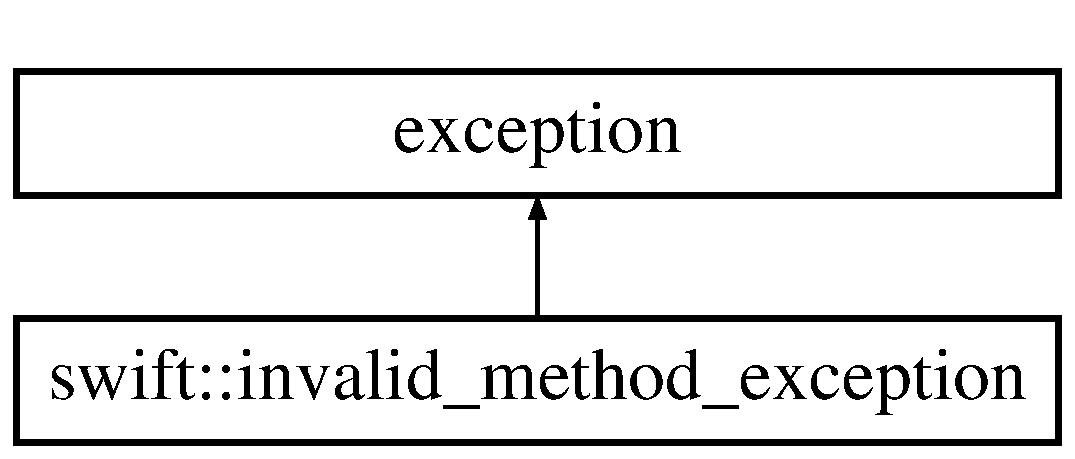
\includegraphics[height=2.000000cm]{classswift_1_1invalid__method__exception}
\end{center}
\end{figure}


The documentation for this class was generated from the following file\-:\begin{DoxyCompactItemize}
\item 
swift.\-cpp\end{DoxyCompactItemize}

\hypertarget{structiobuf}{\section{iobuf Struct Reference}
\label{structiobuf}\index{iobuf@{iobuf}}
}
\subsection*{Public Attributes}
\begin{DoxyCompactItemize}
\item 
\hypertarget{structiobuf_a2ffa253d36125704954f291d3e76dfba}{char $\ast$ {\bfseries buf}}\label{structiobuf_a2ffa253d36125704954f291d3e76dfba}

\item 
\hypertarget{structiobuf_a2f68dd7bfaffe90bce672a38bc863205}{size\-\_\-t {\bfseries len}}\label{structiobuf_a2f68dd7bfaffe90bce672a38bc863205}

\item 
\hypertarget{structiobuf_a2dbeff3cc1ac19c879f92458eff91510}{size\-\_\-t {\bfseries size}}\label{structiobuf_a2dbeff3cc1ac19c879f92458eff91510}

\end{DoxyCompactItemize}


The documentation for this struct was generated from the following file\-:\begin{DoxyCompactItemize}
\item 
mongoose.\-c\end{DoxyCompactItemize}

\hypertarget{struct_m_d5_context}{\section{M\-D5\-Context Struct Reference}
\label{struct_m_d5_context}\index{M\-D5\-Context@{M\-D5\-Context}}
}
\subsection*{Public Attributes}
\begin{DoxyCompactItemize}
\item 
\hypertarget{struct_m_d5_context_a6129b10b90387e1cb1d4cd92e4605c33}{uint32\-\_\-t {\bfseries buf} \mbox{[}4\mbox{]}}\label{struct_m_d5_context_a6129b10b90387e1cb1d4cd92e4605c33}

\item 
\hypertarget{struct_m_d5_context_a48f837fb64afd013f832e3cdab68e5de}{uint32\-\_\-t {\bfseries bits} \mbox{[}2\mbox{]}}\label{struct_m_d5_context_a48f837fb64afd013f832e3cdab68e5de}

\item 
\hypertarget{struct_m_d5_context_ae8be45f236e5cb12b0ae79da77e5f929}{unsigned char {\bfseries in} \mbox{[}64\mbox{]}}\label{struct_m_d5_context_ae8be45f236e5cb12b0ae79da77e5f929}

\end{DoxyCompactItemize}


The documentation for this struct was generated from the following file\-:\begin{DoxyCompactItemize}
\item 
mongoose.\-c\end{DoxyCompactItemize}

\hypertarget{structmg__connection}{\section{mg\-\_\-connection Struct Reference}
\label{structmg__connection}\index{mg\-\_\-connection@{mg\-\_\-connection}}
}
\subsection*{Classes}
\begin{DoxyCompactItemize}
\item 
struct \hyperlink{structmg__connection_1_1mg__header}{mg\-\_\-header}
\end{DoxyCompactItemize}
\subsection*{Public Attributes}
\begin{DoxyCompactItemize}
\item 
\hypertarget{structmg__connection_a7a2b15778b91c5f4654271bc941e5e6f}{const char $\ast$ {\bfseries request\-\_\-method}}\label{structmg__connection_a7a2b15778b91c5f4654271bc941e5e6f}

\item 
\hypertarget{structmg__connection_a65b85efe4e7c90b57a9b7452c5bb7730}{const char $\ast$ {\bfseries uri}}\label{structmg__connection_a65b85efe4e7c90b57a9b7452c5bb7730}

\item 
\hypertarget{structmg__connection_aa2cad585b774df954a8da43b404db695}{const char $\ast$ {\bfseries http\-\_\-version}}\label{structmg__connection_aa2cad585b774df954a8da43b404db695}

\item 
\hypertarget{structmg__connection_a945360c8666acb1546867b9043fb6f61}{const char $\ast$ {\bfseries query\-\_\-string}}\label{structmg__connection_a945360c8666acb1546867b9043fb6f61}

\item 
\hypertarget{structmg__connection_aed0bf0830e52410e0ea6e404aaf19892}{char {\bfseries remote\-\_\-ip} \mbox{[}48\mbox{]}}\label{structmg__connection_aed0bf0830e52410e0ea6e404aaf19892}

\item 
\hypertarget{structmg__connection_a95a74b7afd4c2b1edee0dfa81ef9870b}{char {\bfseries local\-\_\-ip} \mbox{[}48\mbox{]}}\label{structmg__connection_a95a74b7afd4c2b1edee0dfa81ef9870b}

\item 
\hypertarget{structmg__connection_a4420563d43b4f800438585b8b32204e1}{unsigned short {\bfseries remote\-\_\-port}}\label{structmg__connection_a4420563d43b4f800438585b8b32204e1}

\item 
\hypertarget{structmg__connection_a979cee1562ca5e92e561ef82f3842f87}{unsigned short {\bfseries local\-\_\-port}}\label{structmg__connection_a979cee1562ca5e92e561ef82f3842f87}

\item 
\hypertarget{structmg__connection_a48af0c95935d50e2a33fc5dd2c275643}{int {\bfseries num\-\_\-headers}}\label{structmg__connection_a48af0c95935d50e2a33fc5dd2c275643}

\item 
\hypertarget{structmg__connection_a63386f3005373a7b41fe857a8535cf51}{struct \hyperlink{structmg__connection_1_1mg__header}{mg\-\_\-connection\-::mg\-\_\-header} {\bfseries http\-\_\-headers} \mbox{[}30\mbox{]}}\label{structmg__connection_a63386f3005373a7b41fe857a8535cf51}

\item 
\hypertarget{structmg__connection_a817740e63b59b7c45685f1cdb987f98c}{char $\ast$ {\bfseries content}}\label{structmg__connection_a817740e63b59b7c45685f1cdb987f98c}

\item 
\hypertarget{structmg__connection_a6e7a6042a40453587cfca0d325a30601}{size\-\_\-t {\bfseries content\-\_\-len}}\label{structmg__connection_a6e7a6042a40453587cfca0d325a30601}

\item 
\hypertarget{structmg__connection_ad1642e1e64e670e8af715a5aad9e06b0}{int {\bfseries is\-\_\-websocket}}\label{structmg__connection_ad1642e1e64e670e8af715a5aad9e06b0}

\item 
\hypertarget{structmg__connection_ae0163f2496aed16dc972e2139b66bb93}{int {\bfseries status\-\_\-code}}\label{structmg__connection_ae0163f2496aed16dc972e2139b66bb93}

\item 
\hypertarget{structmg__connection_a022231787b07741122d408e9a42a2452}{int {\bfseries wsbits}}\label{structmg__connection_a022231787b07741122d408e9a42a2452}

\item 
\hypertarget{structmg__connection_a1d8ed96e79904e61cbcaa85812c040a8}{void $\ast$ {\bfseries server\-\_\-param}}\label{structmg__connection_a1d8ed96e79904e61cbcaa85812c040a8}

\item 
\hypertarget{structmg__connection_abd930cc6bad9df41986f7c63bddd1d47}{void $\ast$ {\bfseries connection\-\_\-param}}\label{structmg__connection_abd930cc6bad9df41986f7c63bddd1d47}

\item 
\hypertarget{structmg__connection_a767bf7e481bd80da1beabec5e3880c90}{void $\ast$ {\bfseries callback\-\_\-param}}\label{structmg__connection_a767bf7e481bd80da1beabec5e3880c90}

\item 
\hypertarget{structmg__connection_a4bde8827f293f536b64c298b3e00cf1b}{int {\bfseries server\-\_\-id}}\label{structmg__connection_a4bde8827f293f536b64c298b3e00cf1b}

\end{DoxyCompactItemize}


The documentation for this struct was generated from the following file\-:\begin{DoxyCompactItemize}
\item 
mongoose.\-h\end{DoxyCompactItemize}

\hypertarget{structmg__expansion}{\section{mg\-\_\-expansion Struct Reference}
\label{structmg__expansion}\index{mg\-\_\-expansion@{mg\-\_\-expansion}}
}
\subsection*{Public Attributes}
\begin{DoxyCompactItemize}
\item 
\hypertarget{structmg__expansion_a3cc07d545ce1725a6b2e35d9f3ac0d94}{const char $\ast$ {\bfseries keyword}}\label{structmg__expansion_a3cc07d545ce1725a6b2e35d9f3ac0d94}

\item 
\hypertarget{structmg__expansion_a66ecf4f72da0aaf09513053ce1d4bd47}{void($\ast$ {\bfseries handler} )(struct \hyperlink{structmg__connection}{mg\-\_\-connection} $\ast$)}\label{structmg__expansion_a66ecf4f72da0aaf09513053ce1d4bd47}

\end{DoxyCompactItemize}


The documentation for this struct was generated from the following file\-:\begin{DoxyCompactItemize}
\item 
mongoose.\-h\end{DoxyCompactItemize}

\hypertarget{structmg__connection_1_1mg__header}{\section{mg\-\_\-connection\-:\-:mg\-\_\-header Struct Reference}
\label{structmg__connection_1_1mg__header}\index{mg\-\_\-connection\-::mg\-\_\-header@{mg\-\_\-connection\-::mg\-\_\-header}}
}
\subsection*{Public Attributes}
\begin{DoxyCompactItemize}
\item 
\hypertarget{structmg__connection_1_1mg__header_aedc58218d3a1364007fb40c85c77ed38}{const char $\ast$ {\bfseries name}}\label{structmg__connection_1_1mg__header_aedc58218d3a1364007fb40c85c77ed38}

\item 
\hypertarget{structmg__connection_1_1mg__header_af2b60bf6efc5265fceed591c6c2e0741}{const char $\ast$ {\bfseries value}}\label{structmg__connection_1_1mg__header_af2b60bf6efc5265fceed591c6c2e0741}

\end{DoxyCompactItemize}


The documentation for this struct was generated from the following file\-:\begin{DoxyCompactItemize}
\item 
mongoose.\-h\end{DoxyCompactItemize}

\hypertarget{structmg__iterator}{\section{mg\-\_\-iterator Struct Reference}
\label{structmg__iterator}\index{mg\-\_\-iterator@{mg\-\_\-iterator}}
}
\subsection*{Public Attributes}
\begin{DoxyCompactItemize}
\item 
\hypertarget{structmg__iterator_a3da164e715d23835e6c0f21021609c8f}{mg\-\_\-handler\-\_\-t {\bfseries cb}}\label{structmg__iterator_a3da164e715d23835e6c0f21021609c8f}

\item 
\hypertarget{structmg__iterator_a2bb79d73d4b904aa92e89ddd77233dc7}{void $\ast$ {\bfseries param}}\label{structmg__iterator_a2bb79d73d4b904aa92e89ddd77233dc7}

\end{DoxyCompactItemize}


The documentation for this struct was generated from the following file\-:\begin{DoxyCompactItemize}
\item 
mongoose.\-c\end{DoxyCompactItemize}

\hypertarget{structmg__server}{\section{mg\-\_\-server Struct Reference}
\label{structmg__server}\index{mg\-\_\-server@{mg\-\_\-server}}
}
\subsection*{Public Attributes}
\begin{DoxyCompactItemize}
\item 
\hypertarget{structmg__server_aae82596eb59f601ae99ef20f23c12017}{struct \hyperlink{structns__server}{ns\-\_\-server} {\bfseries ns\-\_\-server}}\label{structmg__server_aae82596eb59f601ae99ef20f23c12017}

\item 
\hypertarget{structmg__server_acbc9c742af372629b15619508931d1c5}{union \hyperlink{unionsocket__address}{socket\-\_\-address} {\bfseries lsa}}\label{structmg__server_acbc9c742af372629b15619508931d1c5}

\item 
\hypertarget{structmg__server_af5d370b4300b218d63d7c6a7b4a7791d}{mg\-\_\-handler\-\_\-t {\bfseries event\-\_\-handler}}\label{structmg__server_af5d370b4300b218d63d7c6a7b4a7791d}

\item 
\hypertarget{structmg__server_a873aee94660c99fb7b4a8a872636f619}{char $\ast$ {\bfseries config\-\_\-options} \mbox{[}N\-U\-M\-\_\-\-O\-P\-T\-I\-O\-N\-S\mbox{]}}\label{structmg__server_a873aee94660c99fb7b4a8a872636f619}

\item 
\hypertarget{structmg__server_aa3a9d6adc14027a93c2f3b4288dad82c}{int {\bfseries server\-\_\-id}}\label{structmg__server_aa3a9d6adc14027a93c2f3b4288dad82c}

\end{DoxyCompactItemize}


The documentation for this struct was generated from the following file\-:\begin{DoxyCompactItemize}
\item 
mongoose.\-c\end{DoxyCompactItemize}

\hypertarget{structns__connection}{\section{ns\-\_\-connection Struct Reference}
\label{structns__connection}\index{ns\-\_\-connection@{ns\-\_\-connection}}
}
\subsection*{Public Attributes}
\begin{DoxyCompactItemize}
\item 
\hypertarget{structns__connection_a904d1cde04d0d773000c9da474df3069}{struct \hyperlink{structns__connection}{ns\-\_\-connection} $\ast$ {\bfseries prev}}\label{structns__connection_a904d1cde04d0d773000c9da474df3069}

\item 
\hypertarget{structns__connection_a5ae0b1d1db0ad28c7e533a09dcebcd64}{struct \hyperlink{structns__connection}{ns\-\_\-connection} $\ast$ {\bfseries next}}\label{structns__connection_a5ae0b1d1db0ad28c7e533a09dcebcd64}

\item 
\hypertarget{structns__connection_aa0086348300a1ecf53b25f8973be9535}{struct \hyperlink{structns__server}{ns\-\_\-server} $\ast$ {\bfseries server}}\label{structns__connection_aa0086348300a1ecf53b25f8973be9535}

\item 
\hypertarget{structns__connection_a6a5131aa2ce6cfb7bb7d1ba346014fa5}{sock\-\_\-t {\bfseries sock}}\label{structns__connection_a6a5131aa2ce6cfb7bb7d1ba346014fa5}

\item 
\hypertarget{structns__connection_a2993b03ed9a1740a85655dfe4e3df0fa}{union \hyperlink{unionsocket__address}{socket\-\_\-address} {\bfseries sa}}\label{structns__connection_a2993b03ed9a1740a85655dfe4e3df0fa}

\item 
\hypertarget{structns__connection_a55e16160bc2e7865ed90ce108e91724c}{struct \hyperlink{structiobuf}{iobuf} {\bfseries recv\-\_\-iobuf}}\label{structns__connection_a55e16160bc2e7865ed90ce108e91724c}

\item 
\hypertarget{structns__connection_a8415869449641f4f20387f40abaed4de}{struct \hyperlink{structiobuf}{iobuf} {\bfseries send\-\_\-iobuf}}\label{structns__connection_a8415869449641f4f20387f40abaed4de}

\item 
\hypertarget{structns__connection_a05f3d0c665984d93dd4e8ef7e0c88c88}{S\-S\-L $\ast$ {\bfseries ssl}}\label{structns__connection_a05f3d0c665984d93dd4e8ef7e0c88c88}

\item 
\hypertarget{structns__connection_ace2bc6e8bbec85302ee8ab9351fe8932}{void $\ast$ {\bfseries connection\-\_\-data}}\label{structns__connection_ace2bc6e8bbec85302ee8ab9351fe8932}

\item 
\hypertarget{structns__connection_ac9c1c38e7d8a3b1a21d361ee61683b20}{time\-\_\-t {\bfseries last\-\_\-io\-\_\-time}}\label{structns__connection_ac9c1c38e7d8a3b1a21d361ee61683b20}

\item 
\hypertarget{structns__connection_ac096ae7a3121c09aa68b36dcef2e4116}{unsigned int {\bfseries flags}}\label{structns__connection_ac096ae7a3121c09aa68b36dcef2e4116}

\end{DoxyCompactItemize}


The documentation for this struct was generated from the following file\-:\begin{DoxyCompactItemize}
\item 
mongoose.\-c\end{DoxyCompactItemize}

\hypertarget{structns__server}{\section{ns\-\_\-server Struct Reference}
\label{structns__server}\index{ns\-\_\-server@{ns\-\_\-server}}
}
\subsection*{Public Attributes}
\begin{DoxyCompactItemize}
\item 
\hypertarget{structns__server_af55726087166f7d03aeddc2ba48f2771}{void $\ast$ {\bfseries server\-\_\-data}}\label{structns__server_af55726087166f7d03aeddc2ba48f2771}

\item 
\hypertarget{structns__server_a2f7aebbeb675d926e9261b1f4cd483ec}{sock\-\_\-t {\bfseries listening\-\_\-sock}}\label{structns__server_a2f7aebbeb675d926e9261b1f4cd483ec}

\item 
\hypertarget{structns__server_aa9e4b475a57bb564fd1584584d2a884e}{struct \hyperlink{structns__connection}{ns\-\_\-connection} $\ast$ {\bfseries active\-\_\-connections}}\label{structns__server_aa9e4b475a57bb564fd1584584d2a884e}

\item 
\hypertarget{structns__server_a841af0d6bb158cd8d171ef4fefb05b71}{ns\-\_\-callback\-\_\-t {\bfseries callback}}\label{structns__server_a841af0d6bb158cd8d171ef4fefb05b71}

\item 
\hypertarget{structns__server_a78c0cc9b40b7dc65849f1978c2e52bd7}{S\-S\-L\-\_\-\-C\-T\-X $\ast$ {\bfseries ssl\-\_\-ctx}}\label{structns__server_a78c0cc9b40b7dc65849f1978c2e52bd7}

\item 
\hypertarget{structns__server_a2986e2d7c46e9f549b9f0155740b5890}{S\-S\-L\-\_\-\-C\-T\-X $\ast$ {\bfseries client\-\_\-ssl\-\_\-ctx}}\label{structns__server_a2986e2d7c46e9f549b9f0155740b5890}

\item 
\hypertarget{structns__server_a7c5be118c1ba0a6ee49ee783ce2054a3}{sock\-\_\-t {\bfseries ctl} \mbox{[}2\mbox{]}}\label{structns__server_a7c5be118c1ba0a6ee49ee783ce2054a3}

\item 
\hypertarget{structns__server_a15ea60d811c97305996918a375e26a45}{int {\bfseries server\-\_\-id}}\label{structns__server_a15ea60d811c97305996918a375e26a45}

\end{DoxyCompactItemize}


The documentation for this struct was generated from the following file\-:\begin{DoxyCompactItemize}
\item 
mongoose.\-c\end{DoxyCompactItemize}

\hypertarget{classswift_1_1null__http__version}{\section{swift\-:\-:null\-\_\-http\-\_\-version Class Reference}
\label{classswift_1_1null__http__version}\index{swift\-::null\-\_\-http\-\_\-version@{swift\-::null\-\_\-http\-\_\-version}}
}
Inheritance diagram for swift\-:\-:null\-\_\-http\-\_\-version\-:\begin{figure}[H]
\begin{center}
\leavevmode
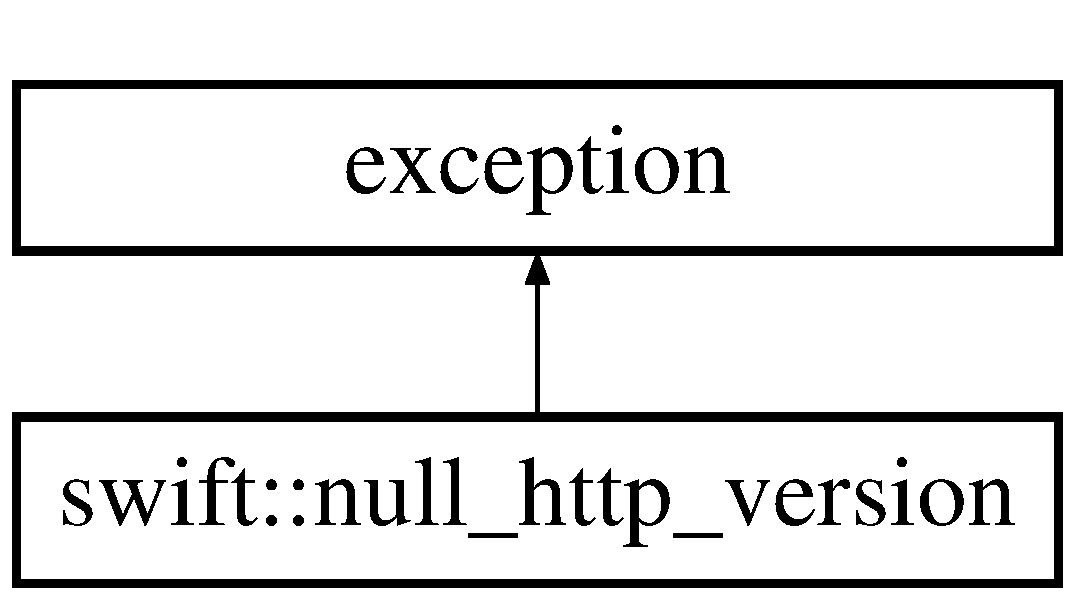
\includegraphics[height=2.000000cm]{classswift_1_1null__http__version}
\end{center}
\end{figure}


The documentation for this class was generated from the following file\-:\begin{DoxyCompactItemize}
\item 
swift.\-cpp\end{DoxyCompactItemize}

\hypertarget{classswift_1_1null__request__exception}{\section{swift\-:\-:null\-\_\-request\-\_\-exception Class Reference}
\label{classswift_1_1null__request__exception}\index{swift\-::null\-\_\-request\-\_\-exception@{swift\-::null\-\_\-request\-\_\-exception}}
}
Inheritance diagram for swift\-:\-:null\-\_\-request\-\_\-exception\-:\begin{figure}[H]
\begin{center}
\leavevmode
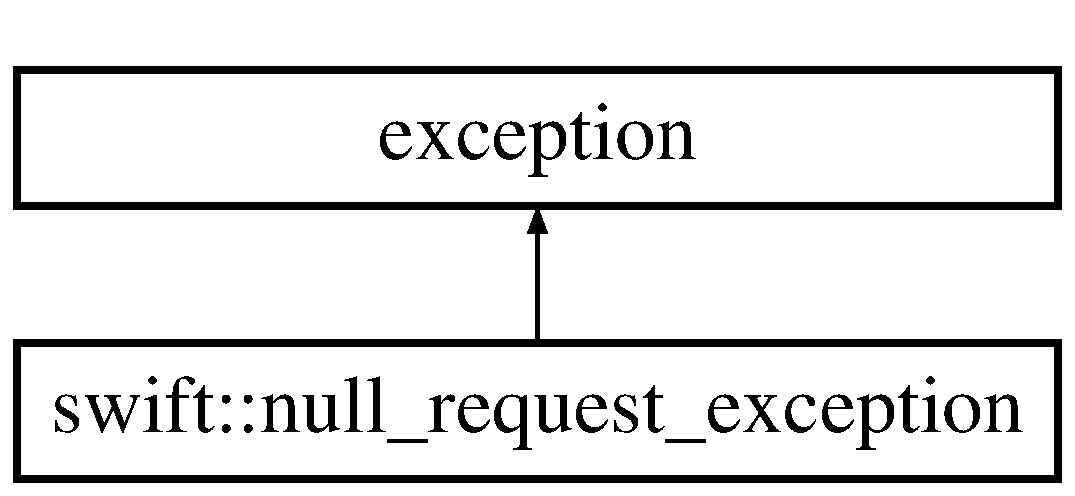
\includegraphics[height=2.000000cm]{classswift_1_1null__request__exception}
\end{center}
\end{figure}


The documentation for this class was generated from the following file\-:\begin{DoxyCompactItemize}
\item 
swift.\-cpp\end{DoxyCompactItemize}

\hypertarget{classswift_1_1null__uri}{\section{swift\-:\-:null\-\_\-uri Class Reference}
\label{classswift_1_1null__uri}\index{swift\-::null\-\_\-uri@{swift\-::null\-\_\-uri}}
}
Inheritance diagram for swift\-:\-:null\-\_\-uri\-:\begin{figure}[H]
\begin{center}
\leavevmode
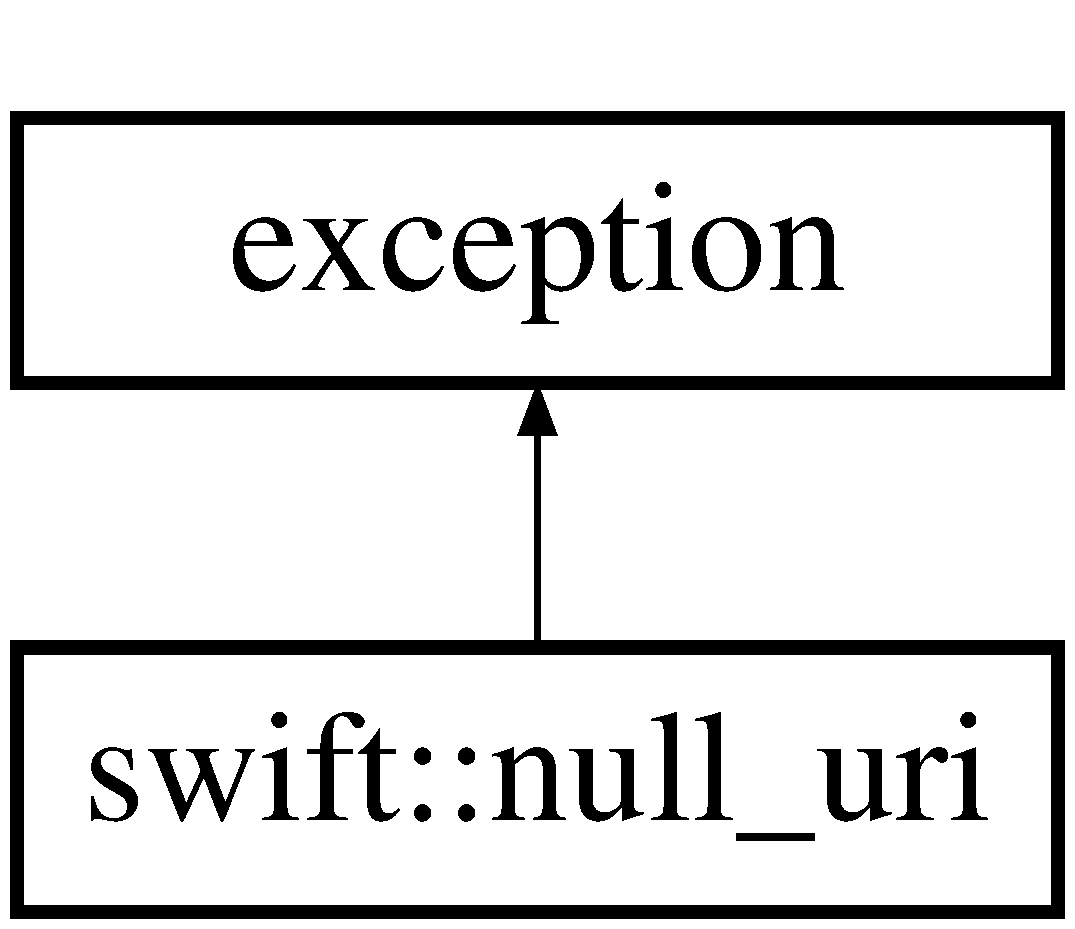
\includegraphics[height=2.000000cm]{classswift_1_1null__uri}
\end{center}
\end{figure}


The documentation for this class was generated from the following file\-:\begin{DoxyCompactItemize}
\item 
swift.\-cpp\end{DoxyCompactItemize}

\hypertarget{classswift_1_1_request}{\section{swift\-:\-:Request Class Reference}
\label{classswift_1_1_request}\index{swift\-::\-Request@{swift\-::\-Request}}
}
\subsection*{Public Member Functions}
\begin{DoxyCompactItemize}
\item 
\hyperlink{classswift_1_1_request_a229fbc0523e779262551de6f4ea2c920}{Request} ()
\item 
\hyperlink{classswift_1_1_request_aede86c57b7c39bc6577a4c4f2f2bf0b8}{Request} (struct \hyperlink{structmg__connection}{mg\-\_\-connection} $\ast$conn)
\item 
\hypertarget{classswift_1_1_request_a328f2b94e10e080c5fd1b6387b71137d}{Method {\bfseries get\-Method} ()}\label{classswift_1_1_request_a328f2b94e10e080c5fd1b6387b71137d}

\item 
\hypertarget{classswift_1_1_request_a65044036527328dd16d663e188ea0a9b}{std\-::string {\bfseries get\-Method\-Str} ()}\label{classswift_1_1_request_a65044036527328dd16d663e188ea0a9b}

\item 
\hypertarget{classswift_1_1_request_adc50d14c9210515e0787efc6085f59c3}{std\-::string {\bfseries get\-U\-R\-I} ()}\label{classswift_1_1_request_adc50d14c9210515e0787efc6085f59c3}

\item 
\hypertarget{classswift_1_1_request_ade67461a7ea078229ec148f16b419395}{std\-::string {\bfseries get\-H\-T\-T\-P\-Version} ()}\label{classswift_1_1_request_ade67461a7ea078229ec148f16b419395}

\item 
\hypertarget{classswift_1_1_request_a271ca3d7daa2541890db65560416443e}{std\-::string {\bfseries get\-Query\-String} ()}\label{classswift_1_1_request_a271ca3d7daa2541890db65560416443e}

\item 
\hypertarget{classswift_1_1_request_a4db2baff092ff72728e6514d990375ca}{std\-::string {\bfseries get\-Remote\-I\-P} ()}\label{classswift_1_1_request_a4db2baff092ff72728e6514d990375ca}

\item 
\hypertarget{classswift_1_1_request_a1feb5c291556a2e5b5a8699a28115ac6}{std\-::string {\bfseries get\-Local\-I\-P} ()}\label{classswift_1_1_request_a1feb5c291556a2e5b5a8699a28115ac6}

\item 
\hypertarget{classswift_1_1_request_aff1e3780cc753fba7f89a8eeb2ea92c2}{unsigned short {\bfseries get\-Remote\-Port} ()}\label{classswift_1_1_request_aff1e3780cc753fba7f89a8eeb2ea92c2}

\item 
\hypertarget{classswift_1_1_request_aacb02c6e51b4fd3cde2bd5d34a28d867}{unsigned short {\bfseries get\-Local\-Port} ()}\label{classswift_1_1_request_aacb02c6e51b4fd3cde2bd5d34a28d867}

\item 
\hypertarget{classswift_1_1_request_a4a9ff6b840751add62789c83034d966c}{std\-::string {\bfseries get\-Content} ()}\label{classswift_1_1_request_a4a9ff6b840751add62789c83034d966c}

\item 
\hypertarget{classswift_1_1_request_adbfa92791e86bea9ec16a0be24ea24f9}{size\-\_\-t {\bfseries get\-Content\-Len} ()}\label{classswift_1_1_request_adbfa92791e86bea9ec16a0be24ea24f9}

\item 
\hypertarget{classswift_1_1_request_a30dcfe1b263feda9c3cd1666e1ad2ff1}{int {\bfseries get\-Header\-Count} ()}\label{classswift_1_1_request_a30dcfe1b263feda9c3cd1666e1ad2ff1}

\end{DoxyCompactItemize}


\subsection{Constructor \& Destructor Documentation}
\hypertarget{classswift_1_1_request_a229fbc0523e779262551de6f4ea2c920}{\index{swift\-::\-Request@{swift\-::\-Request}!Request@{Request}}
\index{Request@{Request}!swift::Request@{swift\-::\-Request}}
\subsubsection[{Request}]{\setlength{\rightskip}{0pt plus 5cm}swift\-::\-Request\-::\-Request (
\begin{DoxyParamCaption}
{}
\end{DoxyParamCaption}
)}}\label{classswift_1_1_request_a229fbc0523e779262551de6f4ea2c920}
Constructs a blank request object \hypertarget{classswift_1_1_request_aede86c57b7c39bc6577a4c4f2f2bf0b8}{\index{swift\-::\-Request@{swift\-::\-Request}!Request@{Request}}
\index{Request@{Request}!swift::Request@{swift\-::\-Request}}
\subsubsection[{Request}]{\setlength{\rightskip}{0pt plus 5cm}swift\-::\-Request\-::\-Request (
\begin{DoxyParamCaption}
\item[{struct {\bf mg\-\_\-connection} $\ast$}]{conn}
\end{DoxyParamCaption}
)}}\label{classswift_1_1_request_aede86c57b7c39bc6577a4c4f2f2bf0b8}
Constructs a \hyperlink{classswift_1_1_request}{Request} object from a Mongoose connection object 

The documentation for this class was generated from the following files\-:\begin{DoxyCompactItemize}
\item 
swift.\-h\item 
swift.\-cpp\end{DoxyCompactItemize}

\hypertarget{classswift_1_1_server}{\section{swift\-:\-:Server Class Reference}
\label{classswift_1_1_server}\index{swift\-::\-Server@{swift\-::\-Server}}
}
\subsection*{Public Member Functions}
\begin{DoxyCompactItemize}
\item 
\hyperlink{classswift_1_1_server_a0322af4ef5852cd53e37dc661c46637b}{Server} ()
\item 
\hyperlink{classswift_1_1_server_aef7faff951fc4b6f82450fd93f7c06c5}{$\sim$\-Server} ()
\item 
void \hyperlink{classswift_1_1_server_aff8c9f94b8d827131b0b80b6607ea01f}{Start} ()
\item 
void \hyperlink{classswift_1_1_server_a9778a55fbf0118a856af782d21562019}{Start} (int port)
\item 
void \hyperlink{classswift_1_1_server_ae4354d31df0a668c8de089da2faf1ab2}{add\-Resource} (std\-::string request\-\_\-path, std\-::string file\-\_\-path)
\item 
void \hyperlink{classswift_1_1_server_ac07ca21b3203f486ae6372d7accfabce}{add\-Resource} (std\-::string request\-\_\-path, std\-::string file\-\_\-path, bool preload)
\item 
void \hyperlink{classswift_1_1_server_adad7a0c0bf0431015333228969957fc4}{add\-Hook} (\hyperlink{classswift_1_1_hook}{Hook} $\ast$hook)
\item 
void \hyperlink{classswift_1_1_server_ad94cc232553cbbddb57463c343456e18}{set\-Cache\-Size} (size\-\_\-t size)
\item 
void \hyperlink{classswift_1_1_server_a689cb1da20caa7c8a5ac733a4259f87b}{set\-Verbose} (bool)
\end{DoxyCompactItemize}
\subsection*{Static Public Member Functions}
\begin{DoxyCompactItemize}
\item 
static \hyperlink{classswift_1_1_server}{Server} $\ast$ \hyperlink{classswift_1_1_server_a305f7482f2229d522a08f1d92b36dea2}{new\-Server} ()
\end{DoxyCompactItemize}


\subsection{Constructor \& Destructor Documentation}
\hypertarget{classswift_1_1_server_a0322af4ef5852cd53e37dc661c46637b}{\index{swift\-::\-Server@{swift\-::\-Server}!Server@{Server}}
\index{Server@{Server}!swift::Server@{swift\-::\-Server}}
\subsubsection[{Server}]{\setlength{\rightskip}{0pt plus 5cm}swift\-::\-Server\-::\-Server (
\begin{DoxyParamCaption}
{}
\end{DoxyParamCaption}
)}}\label{classswift_1_1_server_a0322af4ef5852cd53e37dc661c46637b}
Swift constructor \hypertarget{classswift_1_1_server_aef7faff951fc4b6f82450fd93f7c06c5}{\index{swift\-::\-Server@{swift\-::\-Server}!$\sim$\-Server@{$\sim$\-Server}}
\index{$\sim$\-Server@{$\sim$\-Server}!swift::Server@{swift\-::\-Server}}
\subsubsection[{$\sim$\-Server}]{\setlength{\rightskip}{0pt plus 5cm}swift\-::\-Server\-::$\sim$\-Server (
\begin{DoxyParamCaption}
{}
\end{DoxyParamCaption}
)}}\label{classswift_1_1_server_aef7faff951fc4b6f82450fd93f7c06c5}
Swift destructor 

\subsection{Member Function Documentation}
\hypertarget{classswift_1_1_server_adad7a0c0bf0431015333228969957fc4}{\index{swift\-::\-Server@{swift\-::\-Server}!add\-Hook@{add\-Hook}}
\index{add\-Hook@{add\-Hook}!swift::Server@{swift\-::\-Server}}
\subsubsection[{add\-Hook}]{\setlength{\rightskip}{0pt plus 5cm}void swift\-::\-Server\-::add\-Hook (
\begin{DoxyParamCaption}
\item[{{\bf Hook} $\ast$}]{hook}
\end{DoxyParamCaption}
)}}\label{classswift_1_1_server_adad7a0c0bf0431015333228969957fc4}
Adds an A\-P\-I \hyperlink{classswift_1_1_hook}{Hook} to the server 
\begin{DoxyParams}{Parameters}
{\em hook} & object \\
\hline
\end{DoxyParams}
\hypertarget{classswift_1_1_server_ae4354d31df0a668c8de089da2faf1ab2}{\index{swift\-::\-Server@{swift\-::\-Server}!add\-Resource@{add\-Resource}}
\index{add\-Resource@{add\-Resource}!swift::Server@{swift\-::\-Server}}
\subsubsection[{add\-Resource}]{\setlength{\rightskip}{0pt plus 5cm}void swift\-::\-Server\-::add\-Resource (
\begin{DoxyParamCaption}
\item[{std\-::string}]{request\-\_\-path, }
\item[{std\-::string}]{file\-\_\-path}
\end{DoxyParamCaption}
)}}\label{classswift_1_1_server_ae4354d31df0a668c8de089da2faf1ab2}
Adds a file resource to the server with default settings 
\begin{DoxyParams}{Parameters}
{\em request} & path \\
\hline
{\em file} & path \\
\hline
\end{DoxyParams}
\hypertarget{classswift_1_1_server_ac07ca21b3203f486ae6372d7accfabce}{\index{swift\-::\-Server@{swift\-::\-Server}!add\-Resource@{add\-Resource}}
\index{add\-Resource@{add\-Resource}!swift::Server@{swift\-::\-Server}}
\subsubsection[{add\-Resource}]{\setlength{\rightskip}{0pt plus 5cm}void swift\-::\-Server\-::add\-Resource (
\begin{DoxyParamCaption}
\item[{std\-::string}]{request\-\_\-path, }
\item[{std\-::string}]{file\-\_\-path, }
\item[{bool}]{preload}
\end{DoxyParamCaption}
)}}\label{classswift_1_1_server_ac07ca21b3203f486ae6372d7accfabce}
Adds a file resource to the server 
\begin{DoxyParams}{Parameters}
{\em request} & path \\
\hline
{\em file} & path \\
\hline
{\em preload} & the resource \\
\hline
\end{DoxyParams}
\hypertarget{classswift_1_1_server_a305f7482f2229d522a08f1d92b36dea2}{\index{swift\-::\-Server@{swift\-::\-Server}!new\-Server@{new\-Server}}
\index{new\-Server@{new\-Server}!swift::Server@{swift\-::\-Server}}
\subsubsection[{new\-Server}]{\setlength{\rightskip}{0pt plus 5cm}{\bf Server} $\ast$ swift\-::\-Server\-::new\-Server (
\begin{DoxyParamCaption}
{}
\end{DoxyParamCaption}
)\hspace{0.3cm}{\ttfamily [static]}}}\label{classswift_1_1_server_a305f7482f2229d522a08f1d92b36dea2}
Returns a new swift server object \begin{DoxyReturn}{Returns}
swift server 
\end{DoxyReturn}
\hypertarget{classswift_1_1_server_ad94cc232553cbbddb57463c343456e18}{\index{swift\-::\-Server@{swift\-::\-Server}!set\-Cache\-Size@{set\-Cache\-Size}}
\index{set\-Cache\-Size@{set\-Cache\-Size}!swift::Server@{swift\-::\-Server}}
\subsubsection[{set\-Cache\-Size}]{\setlength{\rightskip}{0pt plus 5cm}void swift\-::\-Server\-::set\-Cache\-Size (
\begin{DoxyParamCaption}
\item[{size\-\_\-t}]{size}
\end{DoxyParamCaption}
)}}\label{classswift_1_1_server_ad94cc232553cbbddb57463c343456e18}
Sets the server's cache size. If it is set at a smaller number than the current usage, the cached files will not be affected. \hypertarget{classswift_1_1_server_a689cb1da20caa7c8a5ac733a4259f87b}{\index{swift\-::\-Server@{swift\-::\-Server}!set\-Verbose@{set\-Verbose}}
\index{set\-Verbose@{set\-Verbose}!swift::Server@{swift\-::\-Server}}
\subsubsection[{set\-Verbose}]{\setlength{\rightskip}{0pt plus 5cm}void swift\-::\-Server\-::set\-Verbose (
\begin{DoxyParamCaption}
\item[{bool}]{}
\end{DoxyParamCaption}
)}}\label{classswift_1_1_server_a689cb1da20caa7c8a5ac733a4259f87b}
Makes Swift verbose \hypertarget{classswift_1_1_server_aff8c9f94b8d827131b0b80b6607ea01f}{\index{swift\-::\-Server@{swift\-::\-Server}!Start@{Start}}
\index{Start@{Start}!swift::Server@{swift\-::\-Server}}
\subsubsection[{Start}]{\setlength{\rightskip}{0pt plus 5cm}void swift\-::\-Server\-::\-Start (
\begin{DoxyParamCaption}
{}
\end{DoxyParamCaption}
)}}\label{classswift_1_1_server_aff8c9f94b8d827131b0b80b6607ea01f}
Starts the server on default port \hypertarget{classswift_1_1_server_a9778a55fbf0118a856af782d21562019}{\index{swift\-::\-Server@{swift\-::\-Server}!Start@{Start}}
\index{Start@{Start}!swift::Server@{swift\-::\-Server}}
\subsubsection[{Start}]{\setlength{\rightskip}{0pt plus 5cm}void swift\-::\-Server\-::\-Start (
\begin{DoxyParamCaption}
\item[{int}]{port}
\end{DoxyParamCaption}
)}}\label{classswift_1_1_server_a9778a55fbf0118a856af782d21562019}
Starts the server on given port 
\begin{DoxyParams}{Parameters}
{\em port} & \\
\hline
\end{DoxyParams}


The documentation for this class was generated from the following files\-:\begin{DoxyCompactItemize}
\item 
swift.\-h\item 
swift.\-cpp\end{DoxyCompactItemize}

\hypertarget{struct_s_h_a1___c_t_x}{\section{S\-H\-A1\-\_\-\-C\-T\-X Struct Reference}
\label{struct_s_h_a1___c_t_x}\index{S\-H\-A1\-\_\-\-C\-T\-X@{S\-H\-A1\-\_\-\-C\-T\-X}}
}
\subsection*{Public Attributes}
\begin{DoxyCompactItemize}
\item 
\hypertarget{struct_s_h_a1___c_t_x_a81d7f6018258ee84f001284c6ff9d2d5}{uint32\-\_\-t {\bfseries state} \mbox{[}5\mbox{]}}\label{struct_s_h_a1___c_t_x_a81d7f6018258ee84f001284c6ff9d2d5}

\item 
\hypertarget{struct_s_h_a1___c_t_x_a7db1dac8c2309a5b22f1cf4bc5de96a5}{uint32\-\_\-t {\bfseries count} \mbox{[}2\mbox{]}}\label{struct_s_h_a1___c_t_x_a7db1dac8c2309a5b22f1cf4bc5de96a5}

\item 
\hypertarget{struct_s_h_a1___c_t_x_a90100b1aab0fedb1d72ded66abeeffe2}{unsigned char {\bfseries buffer} \mbox{[}64\mbox{]}}\label{struct_s_h_a1___c_t_x_a90100b1aab0fedb1d72ded66abeeffe2}

\end{DoxyCompactItemize}


The documentation for this struct was generated from the following file\-:\begin{DoxyCompactItemize}
\item 
mongoose.\-c\end{DoxyCompactItemize}

\hypertarget{unionsocket__address}{\section{socket\-\_\-address Union Reference}
\label{unionsocket__address}\index{socket\-\_\-address@{socket\-\_\-address}}
}
\subsection*{Public Attributes}
\begin{DoxyCompactItemize}
\item 
\hypertarget{unionsocket__address_ab6a9b0bc545e839df7e06e5b6bff0891}{struct sockaddr {\bfseries sa}}\label{unionsocket__address_ab6a9b0bc545e839df7e06e5b6bff0891}

\item 
\hypertarget{unionsocket__address_af540a7224ea459c48bc6ec1ca592e55d}{struct sockaddr\-\_\-in {\bfseries sin}}\label{unionsocket__address_af540a7224ea459c48bc6ec1ca592e55d}

\end{DoxyCompactItemize}


The documentation for this union was generated from the following file\-:\begin{DoxyCompactItemize}
\item 
mongoose.\-c\end{DoxyCompactItemize}

\hypertarget{structvec}{\section{vec Struct Reference}
\label{structvec}\index{vec@{vec}}
}
\subsection*{Public Attributes}
\begin{DoxyCompactItemize}
\item 
\hypertarget{structvec_ae8b8fdc00d1598d046d14d0ae73a441a}{const char $\ast$ {\bfseries ptr}}\label{structvec_ae8b8fdc00d1598d046d14d0ae73a441a}

\item 
\hypertarget{structvec_af52266b373688d591406b7d465ad019c}{int {\bfseries len}}\label{structvec_af52266b373688d591406b7d465ad019c}

\end{DoxyCompactItemize}


The documentation for this struct was generated from the following file\-:\begin{DoxyCompactItemize}
\item 
mongoose.\-c\end{DoxyCompactItemize}

%--- End generated contents ---

% Index
\newpage
\phantomsection
\addcontentsline{toc}{chapter}{Index}
\printindex

\end{document}
